Our study of the gradient flow in the non-linear sigma model consists of computational system to simulate quantum fields numerically. We begin by outlining a numerical Monte Carlo method to simulate the lattice in two and three dimensions. We verify our program with the well-studied $\phi^4$ scalar field theory. We then generalize our model to a vector field to simulate the non-linear sigma model. This simulation system provides data on vacuum states with which we study the gradient flow's effect on topology.

We implement these two algorithms first in Python for the $\phi^4$ model. Afterwards, we transition to C/C++ code due to the increased speed for more complicated theories. For the C++ simulation, we use the \texttt{gcc} compiler with the highest level of optimization.



\section{Fields on the Lattice}
To implement the lattice regularization technique, we must redefine the field action in terms of discrete positions, a process known as ``discretization''. We transition from $x$ as a continuous vector in $\mathbb{R}^2$ to $x_{i,j}$ where
\begin{equation}
    x_{i,j} = ia \hat{\mu}_t + j a \hat{\mu}_x.
\end{equation}
Here, $a$ is the lattice constant and $\hat{\mu}_0$ and $\hat{\mu}_1$ are unit vectors. This change effectively shifts the domain of the field from $\mathbb{R}^2$, which is uncountably infinite, to $\mathbb{Z}^2$, which is countably infinite. To achieve a finite domain, we impose periodic boundary conditions, such that 
\begin{equation}
    \phi\left(x_{i+L,j}\right) = \phi\left(x_{i,j+L}\right) = \phi\left(x_{i,j}\right)
\end{equation}
where $L$ is the side length (in units of the lattice spacing $a$) of the system. In this study we focus solely on square geometries and thus the side length $L$ is unambiguous.

In the $\phi^4$ model, we can specify a discrete action using the Euclidean action from Eq. \ref{eq:phi4 euclidean action}. We begin by redefining the derivative operator as a finite difference:
\begin{align}
    \partial_\mu \phi = \frac{\phi\left(x + a \hat{\mu}\right) - \phi(x)}{a}
\end{align}
We can then define the kinetic term
\begin{align}
    \half \left(\partial_t\phi\right)^2 + \half \left(\partial_x\phi\right)^2 \rightarrow& \frac{1}{2a^2}\left[ \left(\phi(x+a \hat{t}) -\phi(x)\right)^2 + \left(\phi(x+a \hat{x}) -\phi(x)\right)^2\right]\nonumber \\
    \begin{split} \rightarrow& \frac{1}{2a^2}\left[ \phi^2(x+a\hat{t}) + \phi^2(x+a\hat{x}) + 2\phi^2(x)\right.\\ &\qquad \left.- 2\phi(x+a\hat{t})\phi(x) - 2\phi(x+a\hat{x})\phi(x) \right]\hfilneg\end{split}
\end{align}
Since we will eventually sum over all sites $x$, the periodic boundary conditions imply that an overall shift in $x$ does not effect the final action. Therefore, we can combine the first two terms with the third term to produce 
\begin{equation}
    \half \left(\partial_t\phi\right)^2 + \half \left(\partial_x\phi\right)^2 \rightarrow \frac{1}{a^2}\left[ 2\phi^2(x) - \phi(x+a\hat{t})\phi(x) - \phi(x+a\hat{x})\phi(x) \right]
\end{equation}
Unlike the kinetic term, the mass and interaction terms remain unchanged under the discretization procedure. The only remaining change is a shift from an integral to a sum. This takes the form
\begin{equation}
    \label{eq:disc def}
    \int dtdx \rightarrow a^2 \sum_i
\end{equation}
such that the final discretized action becomes
\begin{equation}
    \label{eq:phi4 discretized action}
    S_{\mathrm{lat}}[\phi] = \sum_i \left[-\phi(x_i + a\hat{t})\phi(x_i) - \phi(x_i + a\hat{x})\phi(x_i) + \left(2+\half m_0^2\right)\phi^2(x_i) + \frac{1}{4}\lambda \phi^4(x_i)\right]
\end{equation}

Likewise, we can discretize the non-linear sigma model. In this case, the derivative term becomes 
\begin{equation}
    \half \left(\partial_t\e\right)^2 + \half \left(\partial_x\e\right)^2 \rightarrow \frac{1}{a^2}\left[ 2 - \e(x+a\hat{t})\cdot\e(x) - \e(x+a\hat{x})\cdot\e(x) \right].
\end{equation}
Note that we have used the identity $\e\cdot\e = 1$. Inserting this into Eq.~\ref{eq:nlsm euclidean action} yields the discretized action
\begin{equation}
    \label{eq:nlsm discretized action}
    S_\mathrm{lat}[\e] = \sum_i \left[ 2 - \e(x+a\hat{t})\cdot\e(x) - \e(x+a\hat{x})\cdot\e(x) \right].
\end{equation}

Finally, we redefine the gradient flow in on the lattice. Since the gradient flow is solved exactly in the $\phi^4$ model, we rely on a discrete Fourier Transform. This method isolates the momentum modes of the field and dampens them by a factor of $e^{-\tau p^2}$ where $\tau$ is the flow time and $p$ is the momentum. In the NLSM, the definition of the gradient flow (Eq.~\ref{eq:nsm_gradflow}) becomes 
\begin{equation}
    \label{eq:nsm_gradflow_disc}
    \partial_\tau \e (\tau, x) = \left( 1 - \e(\tau,x) \e(\tau,x)^T\right) \partial^2 \e(\tau,x),
\end{equation}
 where the Laplacian operator $\partial^2$ is defined as
\begin{equation*}
    \partial^2 \e(\tau,x) = \e(\tau, x+a \hat{t}) + \e(\tau,x-a\hat t) + \e(\tau, x+a \hat{x}) + \e(\tau,x-a\hat x) - 4 \e(t)_x.
\end{equation*}
Unlike the $\phi^4$ gradient flow, this differential equation has no analytic solution. Therefore, we numerically solve for the gradient flow using a fourth-order Runge-Kutta approximation (see Sec.~\ref{sec:runga-kutta}).

\subsection{Discretized Observables}
Following the definitions in Sec.~\ref{sec:primary observables}, we redefine the primary and secondary observables on the discretized lattice. Using the discretization definition in Eq.~\ref{eq:disc def}, we express the average magnetization as 
\begin{equation}
|\bar\phi| \equiv \frac{1}{L^2}\left| \sum_i^{L^2} \phi(x_i)\right|.
\end{equation}
in the $\phi^4$ model and 
\begin{equation}
    |\bar\e| \equiv \frac{1}{L^2}\left|\sum_i^{L^2} \e(x_i)\right|.
\end{equation}
in the NLSM, where $L^2 = V/a^2$.

We can also simplify the expression for the magnetic susceptibility. Due to the spin-flip invariance of both fields, the second terms in Eq.~\ref{eq:chim nlsm} and Eq.~\ref{eq:chim phi4} disappear (see Sec.~\ref{sec:avg mag}). In the NLSM, the susceptibility therefore becomes
\begin{align}
    \chi_m &= L^2 \left\langle \left( \sum_x e(x) \right)^2\right\rangle  \\
           &= L^2 \left\langle \sum_{x,y}\e(x)\cdot \e(y) \right\rangle. 
\end{align}
Due to translational invariance from the periodic boundary conditions, we simplify this expression to be
\begin{equation}
    \chi_m = \left\langle \sum_x \e(0)\cdot\e(x) \right\rangle.
\end{equation}
Following the same logic, we derive 
\begin{equation}
    \chi_m = \left\langle \sum_x \phi(0)\phi(x) \right\rangle
\end{equation}
for the $\phi^4$ model. 

The definitions for the internal energy, Binder cumulant and bimodality remain unchanged on the lattice.

\section{Defining the topological charge}
On the lattice, the topological charge is nontrivial to calculate. Primarily, there are multiple possible mappings between field configurations and the integers. In this work, we use the definition found in \cite{berg1981}. To begin, we define a local topological charge density $q$, defined for each square of adjacent lattice points. This square, known as a \textit{plaquette}, is denoted $x^*$. The global charge $Q$ is the sum of all local charges:
\begin{equation}
    Q \equiv \sum_{x^*} q(x^*).
\end{equation}
As a function of $x^*$, the charge density is a function of the field on the plaquette vertices, an idea visualized in Fig.~\ref{fig:plaquette}.
\begin{figure}
    \centering
    \begin{tikzpicture}
        \draw[step=4cm,gray,thin] (-2,-2) grid (6,6);
        \draw[dotted] (0,0) -- (4,4);
        \draw[thick](0,0) node[circle,fill,inner sep=0pt, minimum size=0.3cm]{} node[anchor=north west] {$x_1$} -- 
                    (0,4) node[circle,fill,inner sep=0pt, minimum size=0.3cm]{} node[anchor=north west] {$x_2$} -- 
                    (4,4) node[circle,fill,inner sep=0pt, minimum size=0.3cm]{} node[anchor=north west] {$x_3$} -- 
                    (4,0) node[circle,fill,inner sep=0pt, minimum size=0.3cm]{} node[anchor=north west] {$x_4$} -- cycle ;
                    \draw[] (2,2) node[circle,fill,inner sep=0pt, minimum size=0.3cm]{} node[anchor=north east]{$x^*$};


        \draw[-stealth] (0.2,1) -- (0.2,3);
        \draw[-stealth] (1,3.8) -- (3,3.8);
        \draw[-stealth] (3,3.5) -- (1,1.5);

        \draw[-stealth] (1,0.5) -- (3,2.5);
        \draw[-stealth] (3.8,3) -- (3.8,1);
        \draw[-stealth] (3,0.2) -- (1,0.2);
    \end{tikzpicture}
    \caption{\label{fig:plaquette} Visualization of plaquette $x^*$. Dotted line separated plaquette into two signed areas which are used to define the topological charge density $q(x^*)$. Arrows represent order of signed area.}
\end{figure}
In the NLSM, the field at each of these vertices is a point on the sphere $S^2$. Therefore, there is a signed area $A$ on the sphere associated with each triplet of points, as shown in Fig.~\ref{fig:sphere} (the sign changes with odd permutations of the ordering). We follow the derivation in \cite{berg1981} and split the plaquette into two triangles, as shown in Fig.~\ref{fig:plaquette}, with the ordering determining the sign. The topological charge density is defined using this signed area as
\begin{equation}
    q(x^*) = \frac{1}{4\pi} \bigg[A\Big(\e(x_1), \e(x_3), \e(x_3)\Big) + A\Big(\e(x_1), \e(x_3), \e(x_4)\Big) \bigg].
\end{equation}
This sign is defined if $A\neq 0, 2\pi$, or in other words, as long as the three points on the sphere are distinct and do not form a hemisphere. In numerical calculations, these points can be ignored. Therefore, we impose that the signed area is defined on the smallest spherical triangle, or mathematically
\begin{equation}
    -2\pi < A < 2\pi.
\end{equation}


Following \cite{berg1981}, this yields an expression for the signed area
\begin{equation}
    A(\e_1, \e_2, \e_1) = 2 \:\mathrm{arg}\Big(1+\e_1\cdot\e_2 + \e_2\cdot\e_3 + \e_3\cdot\e_1 + i\e_1 \cdot (\e_2\times\e_3)\Big).
\end{equation}
Under periodic boundary conditions, these triangles on the sphere necessarily wrap $S^2$ an integer number of times, ensuring $Q$ is an integer. In the continuum limit, field must be uniform at $x\rightarrow\infty$ and therefore effectively forms a sphere (see Sec.~\ref{sec:topological charge}).
\begin{figure}[h]
\centering
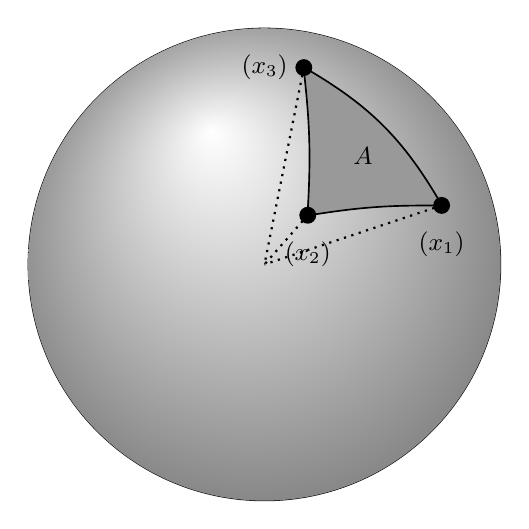
\begin{tikzpicture}
    \pgfdeclarelayer{nodelayer}
    \pgfdeclarelayer{edgelayer}
    \pgfdeclareradialshading{sphere4}{\pgfpoint{-0.2cm}{0.5cm}}% 
        {rgb(0cm)=(1,1,1);
        rgb(1cm)=(0.5,0.5,0.5); rgb(1.05cm)=(1,1,1)}
        %rgb(0.7cm)=(0.1,0.1,0.1); rgb(1cm)=(0.5,0.05,0); rgb(1.05cm)=(1,1,1)}
    \pgfsetlayers{nodelayer,edgelayer}
    \tikzstyle{label}=[fill=none, draw=none, shape=circle]
    \tikzstyle{point}=[inner sep=0pt, minimum size=0.2cm,fill=black, draw, shape=circle]
    %\tikzstyle{interior line}=[{Stealth[scale=1.5]}-,dotted,thick]
    \tikzstyle{interior line}=[dotted,thick]

    \tikzstyle{triangle}=[thick]
    \tikzstyle{arrow}=[->, thick]
	\begin{pgfonlayer}{nodelayer}
		\node [style=point] (4) at (0.5, 2.5) {};
		\node [style=point] (5) at (0.55, 0.625) {};
		\node [style=point] (6) at (2.25, 0.75) {};
		\node (7) at (0, 0) {};
		\node (8) at (1.25, 1.375) {};
		\node (9) at (2.425, 2.525) {};
	\end{pgfonlayer}
	\begin{pgfonlayer}{edgelayer}
        \draw (0,0) circle (3cm);
        %\shade[inner color=white,outer color=lightgray] (0,0) circle (3cm);
        \shade[shading=sphere4] (0,0) circle (3cm);
		\draw [bend left=15,style=triangle] (4.center) to (6.center);
		\draw [bend left=355,style=triangle] (6.center) to (5.center);
		\draw [bend right=5,style=triangle] (5.center) to (4.center);
		\draw [style=interior line] (4.center) to (7.center);
		\draw [style=interior line] (5.center) to (7.center);
        \draw [style=interior line] (6.center) to (7.center);
        \draw [fill=gray!80] (4.center) to [bend left=15] (6.center) to [bend left=355] (5.center) to [bend right=5] cycle;

		%\draw [style=arrow] (8.center) to (9.center);

        \node [style=label, anchor=north] at (2.25, 0.75) {\small $\e(x_1)$};
        \node [style=label, anchor=north] at (0.55, 0.625) {\small $\e(x_2)$};
        \node [style=label, anchor=east] at (0.5, 2.5) {\small $\e(x_3)$};
		\node [style=point] at (4){};
		\node [style=point] at (5){};
		\node [style=point] at (6){};

        \node [style=label] at (8) {\small $A$};
	\end{pgfonlayer}
\end{tikzpicture}
\caption{\label{fig:sphere} Visualization of signed area $A$ on the sphere $S^2$ traced out by field at points $x_1$, $x_2$ and $x_3$.}
\end{figure}
In the NLSM described by Eq.~\ref{eq:nlsm discretized action}, the values of $Q$ are roughly Gaussian around $Q=0$, as shown in Fig.~\ref{fig:hist}.
\begin{figure}[h]
    \centering
      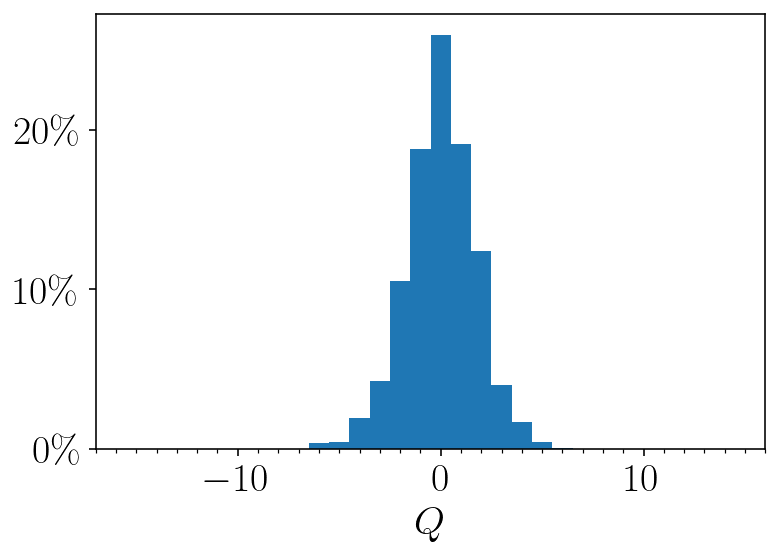
\includegraphics[width=0.6\textwidth]{imgs/hist.png}
      \caption{\label{fig:hist} Histogram of topological charge values $Q$ for trivial NLSM. $L=404$, 10,000 measurements, measurements very 50 sweeps, 1,000 sweep thermalization, $\tau=0$}
\end{figure}

Following this quantity, we can define a topological susceptibility $\chi_t$
\begin{equation}
\chi_t \equiv \frac{1}{L^2} \Big( \langle Q^2 \rangle - \langle Q \rangle^2 \Big).
\end{equation}
In the trivial case, $\langle Q \rangle$ is equal to $0$ and   
\begin{equation}
    \chi_t = \frac{1}{L^2} \sum_{x,y} \langle q(x)q(y)\rangle.
\end{equation}
Assuming periodic boundary conditions and therefore translational symmetry, this expression simplifies to 
\begin{equation}
    \chi_t = \frac{1}{L^2} \sum_{x} \langle q(x)q(0)\rangle.
\end{equation}

On the lattice, this quantity is known to diverge in the continuum limit owing solely to the $x=0$ term \cite{bietenholz2018}. This divergence exists in QCD as well \cite{bruno2014}.


\section{Monte Carlo Simulations}
\label{sec:mc}
We implement a Markov Chain Monte Carlo method following Schaich's thesis \cite{schaich2006}. This implementation utilizes a ``random walk,'' i.e. a set of random steps through phase space, to determine statistical values such as correlation functions across the lattice. By the definition of the Markov chain, the probability of adoption of each state, and therefore its inclusion in the Monte Carlo calculation, depends only on the current state and the proposed state. This probability is denoted as $P(\mu\rightarrow\nu)$ where $\mu$ and $\nu$ are the existing and proposed lattice configurations respectively.

We begin this random walk with a so-called ``hot start'' where each field value at each lattice site is randomly selected. As an alternative to the hot start, we could use a ``cold start'' where the field begins completely aligned. With an appropriate thermalization, these initial configurations have no effect on the Monte Carlo statistics, a fact we verify in Sec.~\ref{sec:thermalization}. 

\subsection{Metropolis Algorithm}
We primarily use the Metropolis algorithm for the calculation of new Markov chain configurations. The method begins with proposing a new value for a single lattice point, which is accepted with a probability
\begin{equation}
    P(\phi_a\rightarrow\phi_b) = \begin{cases} 
        e^{-(S[\phi_b] - S[\phi_a])} & S[\phi_b] < S_[\phi_a] \\
        1 & \mathrm{otherwise} \\
   \end{cases}
\end{equation}
where $\phi_a$ is the initial configuration and $\phi_b$ is the proposed configuration. This process is performed for each point on the lattice, making up a ``sweep''. Repeating this sweep many times pushes the lattice toward the action minimum.


\subsection{Wolff Cluster Algorithm}
Though the Metropolis algorithm will slowly find the absolute minimum of the theory, the presence of local minima can greatly prolong the convergence. Both the $\phi^4$ model and the non-linear sigma model feature ``kinetic'' terms with gradients of $\phi$. Therefore, the presence of large similarly-valued regions in the lattice can lead to a local minimum. One method of removing these clusters involves identifying all clusters on the lattice and probabilistically flipping each, a technique known as the Swendsen-Wang algorithm \cite{swendsen1987}. 

A more efficient approach is the Wolff algorithm \cite{wolff1989}, which \textit{grows} one cluster probabilistically and flips it unconditionally. In the case of $\phi^4$ theory, this flipping takes the form of a simple sign change. In the non-linear sigma model we choose a random unit vector $\vec r$ and consider the projection of the field on this vector. When the cluster flips, each site is flipped along this direction. To identify the cluster, the algorithm uses a recursive algorithm defined by the probability of adding a new site, growing the cluster from a single, randomly selected ``seed''. Starting with the seed, the probability of adding each neighboring site is given by the source site $x$ and the proposed site $x'$. Wolff defines this probability for arbitrary sigma models as 
\begin{equation}
    \label{eq:phi4 wolff padd}
    P_{add}(\e(x),\e(x')) = \begin{cases} 
        1 - e^{2\beta [\vec{r} \cdot \e(x)][\vec{r} \cdot \e(x')]} & \mathrm{sgn}[\vec{r}\cdot\e(x)]=\mathrm{sgn}[\vec{r}\cdot\e(x')]\\
        0 & \mathrm{otherwise} \\
   \end{cases}
\end{equation}
This expression is designed to preserve the detailed balance equations. We can demonstrate this quality, and motivate an equivalent expression for the $\phi^4$ model, by considering the probability $P(\phi\rightarrow f_C(\phi))$ of flipping some cluster $C$. Generally,
\begin{equation}
    P\big(\phi \rightarrow f_C\left(\phi\right)\big) \propto \prod_{\langle x,x'\rangle \in \partial C}  \Big[1 - P_{add}\big(\e(x),\e(x')\big)\Big]
\end{equation}
where $\partial C$ is the set of pairs of sites on the boundary of $C$. Since $P_{add}=0$ for unaligned sites, these pairs contribute nothing to the value. We can also find the probability $P(f_C(\phi) \rightarrow \phi)$ with the same expression:
\begin{equation}
P\big(f_C(\phi)\rightarrow \phi \big) \propto \prod_{\langle x,x'\rangle \in \partial C}  \Big[1 - P_{add}\big(\e(x),R\;\e(x')\big)\Big],
\end{equation}
where the matrix $R$ which is a reflection matrix along the vector $\vec{r}$.

From the discretized action of the NLSM model (Eq.~\ref{eq:nlsm discretized action}) and the detailed balance equation (Eq.~\ref{eq:detailedbalance2}), we derive
\begin{equation}
    \prod_{\langle x,x'\rangle \in \partial C}  \frac{ 1 - P_{add}\big(\e(x),\e(x')\big)}{ 1 - P_{add}\big(\e(x),R\;\e(x')\big)}  = \mathrm{exp}\left\{\beta\sum_{\langle x,x'\rangle \in \partial C} \e(x)\cdot[R-1]\e(x')\right\}.
\end{equation}
Note that all the pairs within and outside the cluster cancel in the fraction on the left and the difference on the right. Using the definition of the reflection matrix
\begin{equation}
    R\,\e = \e - 2(\e\cdot\vec{r})\e,
\end{equation}
we can simplify the equation to be 
\begin{equation}
    \prod_{\langle x,x'\rangle \in \partial C}  \frac{ 1 - P_{add}\big(\e(x),\e(x')\big)}{ 1 - P_{add}\big(\e(x),R\;\e(x')\big)}  = \prod_{\langle x,x'\rangle \in \partial C}\mathrm{exp}\big\{2\beta[r\cdot\e(x)][r\cdot\e(x')]\big\}.
\end{equation}
By plugging in Eq.~\ref{eq:phi4 wolff padd}, it is clear to see this equation is satisfied.

Using this same reasoning, we can deduce an expression for $P_{add}$ in the $\phi^4$ model. Since this model is one dimensional, the reflection matrix $R$ is equivalent to $-1$. Adapting the NLSM detailed balance equation for the $\phi$ field, we find
\begin{equation}
    \prod_{\langle x,x'\rangle \in \partial C}  \frac{ 1 - P_{add}\big(\phi(x),\phi(x')\big)}{ 1 - P_{add}\big(\phi(x),-\phi(x')\big)}  = \prod_{\langle x,x'\rangle \in \partial C}\mathrm{exp}\{-2 \phi(x)\phi(x')\}.
\end{equation}
This equation is satisfied by the ansatz
\begin{equation}
    \label{eq:nlsm wolff padd}
    P_{add}(\phi(x),\phi(x')) = \begin{cases} 
        1 - e^{-2\phi(x)\phi(x')} & \mathrm{sgn}[\phi(x)]=\mathrm{sgn}[\phi(x')]\\
        0 & \mathrm{otherwise} \\
   \end{cases}.
\end{equation}
We will use this expression in the computational implementation of this algorithm.

Fig.~\ref{fig:wolff} shows a real demonstration of this process. We can see a large cluster of negative field values becoming positive. Note that periodic boundary conditions apply, so the small island of black at the bottom is actually part of the larger cluster. Furthermore, this visualization demonstrates the probabilistic nature of the Wolff algorithm. Since states are added probabilistically, there are some small holes in the cluster. These will be removed by following Metropolis sweeps.
\begin{figure}[h]
  \centering
      \begin{subfigure}[b]{0.5\textwidth}\centering
        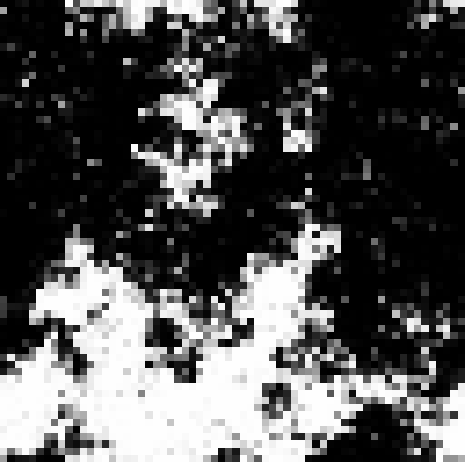
\includegraphics[width=0.6\textwidth]{imgs/wolffa.png}
        \caption{before cluster flip}
      \end{subfigure}%
      \hfill
      \begin{subfigure}[b]{0.5\textwidth}\centering
        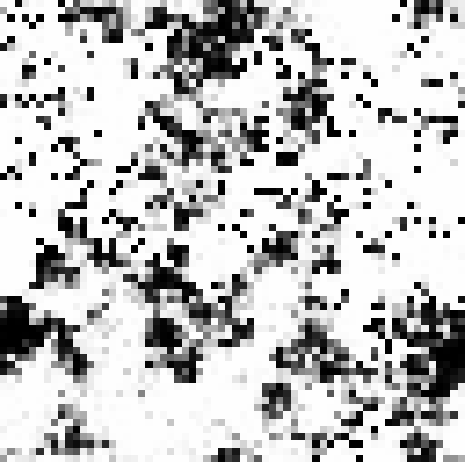
\includegraphics[width=0.6\textwidth]{imgs/wolffb.png}
        \caption{after cluster flip}
      \end{subfigure}
      \hfill
      \caption{\label{fig:wolff} An example of the Wolff cluster algorithm in the $\phi^4$ model. White represents positive values of $\phi$ while black represents negative. $\lambda=0.5$, $m_0^2=-0.9$}
  
\end{figure}

\subsection{Checkerboard algorithm}

In order to parallelize the Metropolis algorithm, we use a checkerboard algorithm. We begin by splitting the lattice into ``white'' sites and ``black'' sites, like the tiles on a checkerboard. Since the Lagrangian density at each site does not depend on diagonal neighbors, each white site is independent of every other white site and likewise for black sites. Therefore, we can split the sites of each color into separate parallel processing nodes and independently run the Metropolis algorithm, ensuring that no site affects the Lagrangian density at any other site. We use this method to parallelize the code through the Message Passing Interface (MPI).

\subsection{Thermalization}
\label{sec:thermalization}
In order to determine the necessary thermalization, we plot the action as a function of Metropolis sweeps in Fig.~\ref{fig:therm}.
\begin{figure}[h]
  \centering
      \begin{subfigure}[b]{0.5\textwidth}\centering
        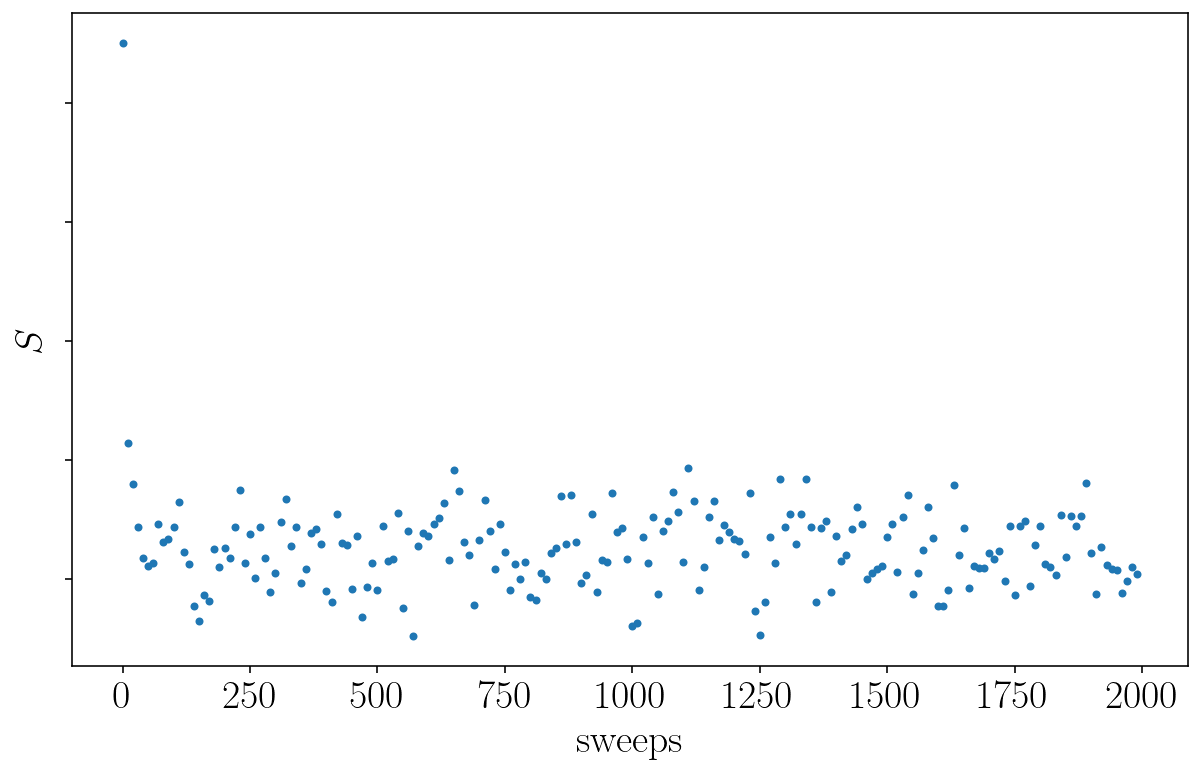
\includegraphics[width=\textwidth]{imgs/therm24.png}
        \caption{$L=24$}
      \end{subfigure}%
      \hfill
      \begin{subfigure}[b]{0.5\textwidth}\centering
        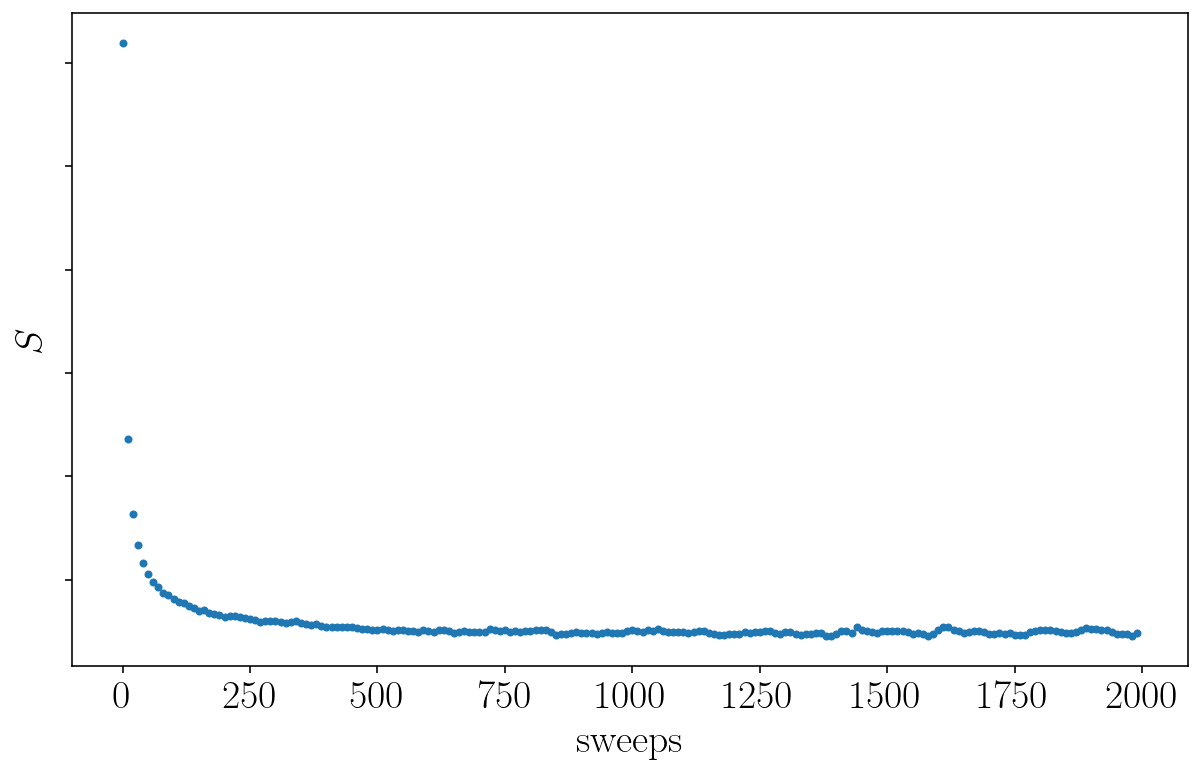
\includegraphics[width=\textwidth]{imgs/therm404.png}
        \caption{$L=404$}
      \end{subfigure}
      \hfill
      \caption{\label{fig:therm} Plots of the action as a function of Monte Carlo time, starting with a random NLSM lattice.}
\end{figure}
Based on this plot, we determine that 1000 sweeps will give sufficient time for the system to reach the classical action minimum. We use this value for the remainder of this study.

We also compare the hot and cold starts by plotting a histogram of the actions in Fig.~\ref{fig:coldstart}. This plot qualitatively demonstrates the irrelevance of the initial configuration.
\begin{figure}[h]
  \centering
    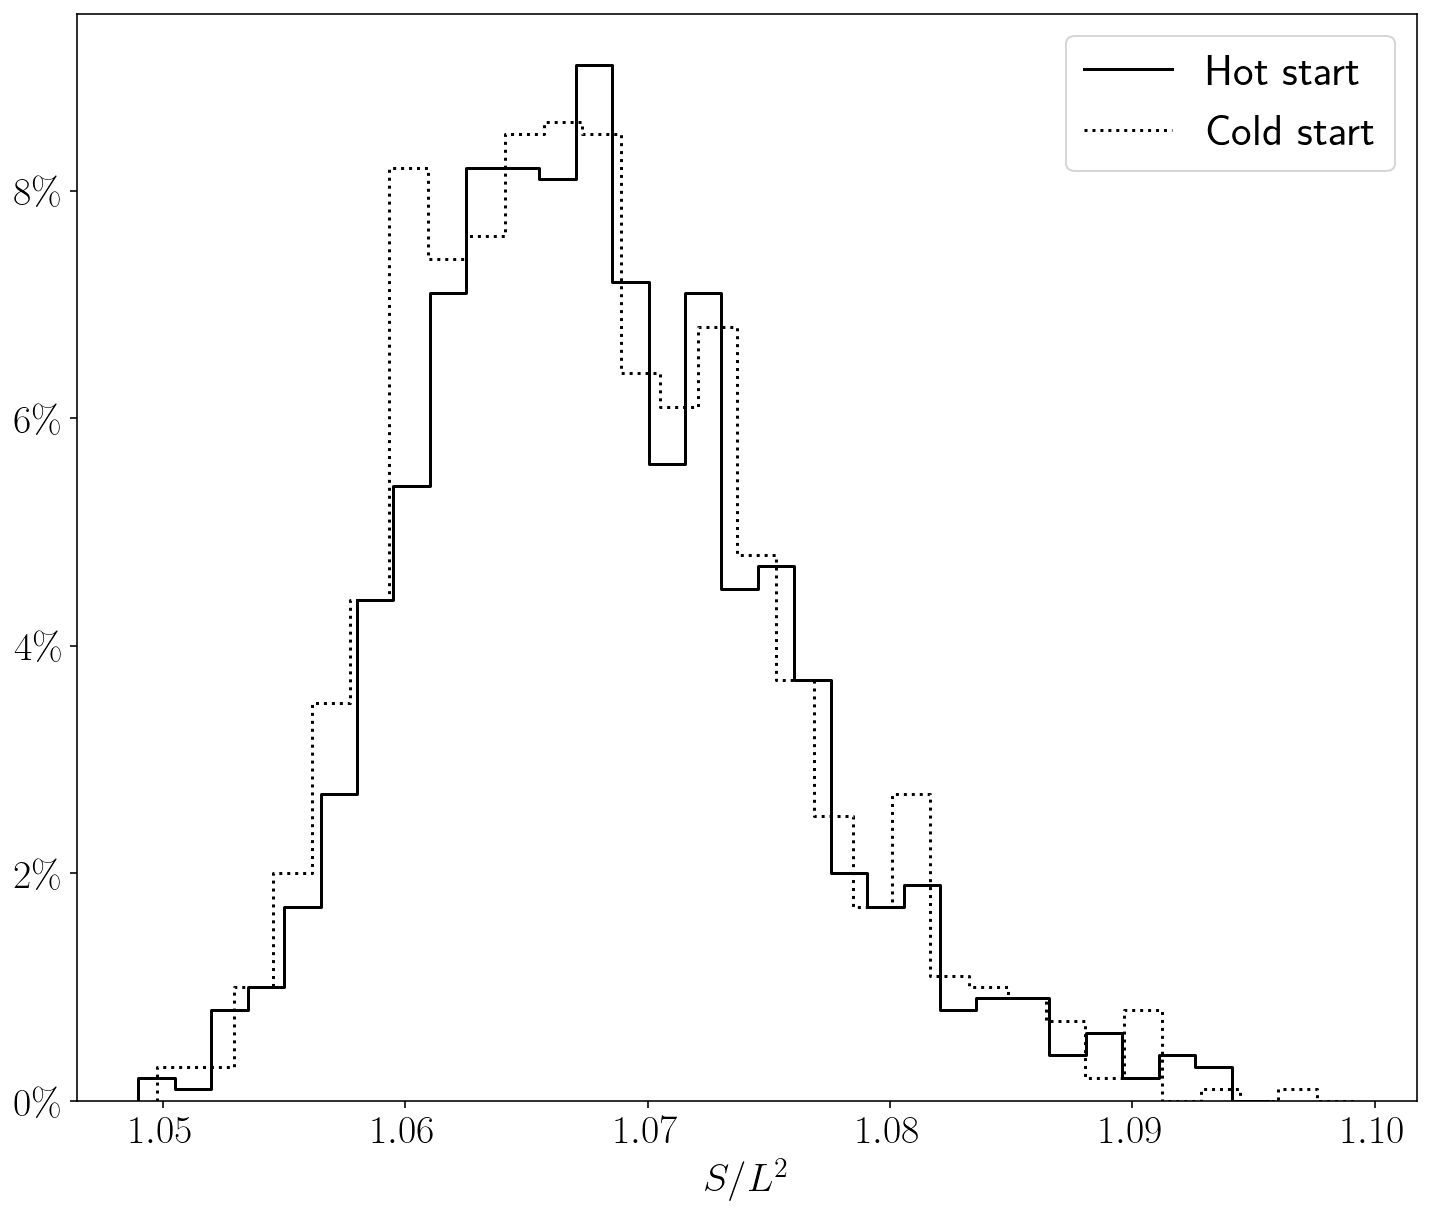
\includegraphics[width=0.6\textwidth]{imgs/coldstart.png}
  \caption{\label{fig:coldstart} Histogram of lattice-averaged actions $S/L^2$ with hot and cold starts. 1,000 sweep thermalization in $L=404$ lattice, 1,000 measurements taken every 50 sweeps.}
\end{figure}

\subsection{Autocorrelation}
Due to the nature of the Markov chain, each member of the ensemble is correlated to every other. Since each configuration is based on previous configurations, each pair of members in the Markov chain has a correlation which decreases exponentially based on the number of steps between. This value is known as the ``autocorrelation'' and scales as $e^{t/\tau_{int}}$ where $t$ is the number of steps between configurations and $\tau_{int}$ is the autocorrelation time.\footnote{Though it is called a time, $\tau_{int}$ is in units of Markov Chain steps.} When performing simulations of the lattice, the number of sweeps between measurements should be much larger than $\tau_{int}$ since Monte Carlo methods generally assume independent observations.

We use Wolff's automatic windowing procedure \cite{wolff2007} and the magnetic susceptibility $\chi_m$ to estimate the autocorrelation. Using Wolff's public MatLab code\footnote{\url{https://www.physik.hu-berlin.de/de/com/ALPHAsoft}}, we estimate the autocorrelation time for $L=24$ and $L=404$ lattices. This algorithm identifies the optimal window size with which to calculate the autocorrelation time. We perform this process on $L=24$ and $L=404$ lattices using a thermalization of $1000$ sweeps and $500$ total measurements. Note that this calculation included a Wolff cluster algorithm every $5$ sweeps. The result of this calculation is shown in Fig.~\ref{fig:tauint}.
\begin{figure}[h]
  \centering
      \begin{subfigure}[b]{0.5\textwidth}\centering
        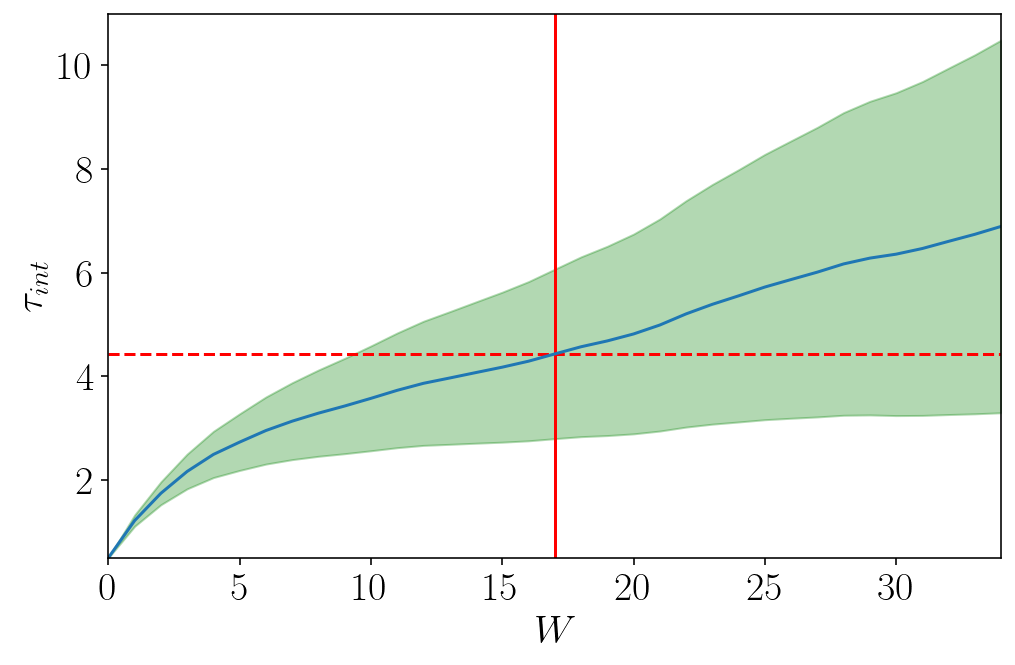
\includegraphics[width=0.9\textwidth]{imgs/tauint24.png}
        \caption{$L=24$, $\tau_{int}=4.43$}
      \end{subfigure}%
      \hfill
      \begin{subfigure}[b]{0.5\textwidth}\centering
        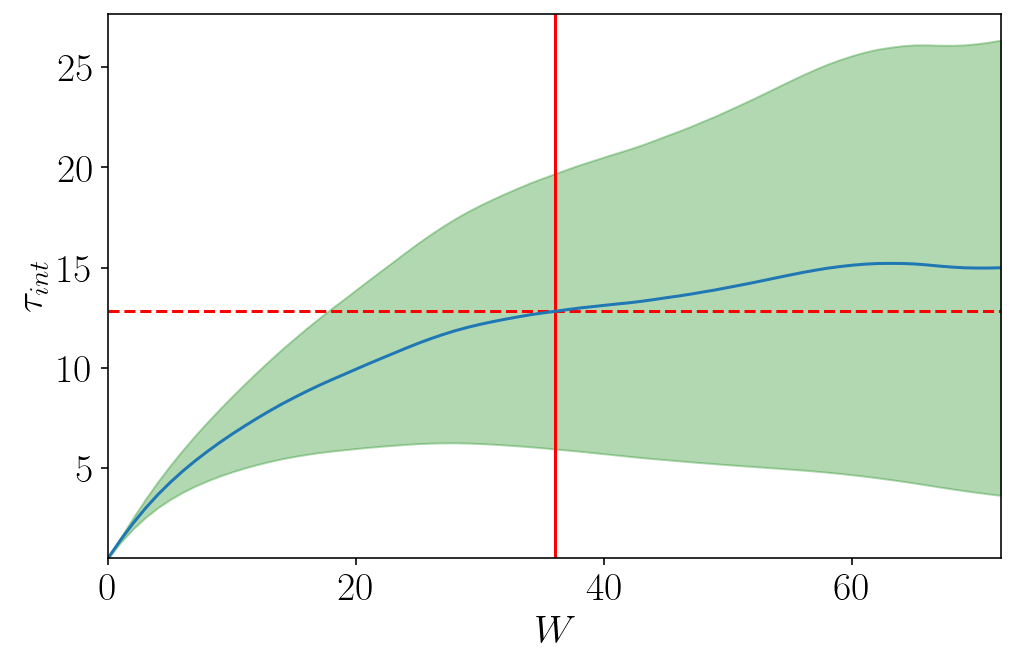
\includegraphics[width=0.9\textwidth]{imgs/tauint404.png}
        \caption{$L=404$, $\tau_{int}=12.81$}
      \end{subfigure}
      \hfill
      \caption{\label{fig:tauint} Plots of automatic windowing procedure used to calculate $\tau_{int}$ for the NLSM model.}
\end{figure}

Based on these two values for $\tau_{int}$, we decide to measure every $50$ sweeps for each simulation. This value will ensure that each measurement is effectively independent.

\subsection{Runge-Kutta Algorithm}
\label{sec:runga-kutta}
In order to calculate the gradient flow, we numerically solve the differential equation using a fourth-order Runga-Kutta approximation. This algorithm refines the Euler method 
\begin{equation*}
    \e(\tau+h,x) \approx \e(\tau)_x + h f(\e(\tau,x))
\end{equation*}
where $f(\e)$ is defined for convenience as 
\begin{equation}
    f(\e)=\partial_\tau \e (\tau,x)  = \left( 1 - \e(\tau,x) \e(\tau,x)^T\right) \partial^2 \e(\tau,x),
\end{equation}
following from Eq.~\ref{eq:nsm_gradflow_disc}. To the fourth order, this approximation becomes 
%
\begin{align}
    \label{eq:rungekutta}
    k_1 &= h f\left(\e\left(\tau,x\right)\right) \\ 
    k_2 &= h f\left(\e\left(\tau,x\right) + \frac{k_1}{2}\right) \\ 
    k_3 &= h f\left(\e\left(\tau,x\right) + \frac{k_2}{2}\right) \\ 
    k_4 &= h f\left(\e\left(\tau,x\right) + k_3\right) \\ 
    \e(\tau+h)_x &= \e(\tau,x) + \frac{k_1}{6} + \frac{k_2}{3} + \frac{k_3}{3} + \frac{k_4}{6} + O(h^5).
\end{align}
This method is usually superior to Euler's method and the midpoint method \cite{vetterling1992}.

To increase the efficiency of this algorithm, we implement the step-doubling algorithm to adaptively adjust $h$. If the error of a Runge-Kutta step is greater than the tolerance, the same step is repeated with half the step size. Alternatively, if the error is less than half of the tolerance, the step size is doubled for the next calculation. Finally, if the step size is greater than the distance to the next measurement, that distance is used as the step size, using the normal value afterwards. Otherwise, the algorithm proceeds with the consistent step size. 


\section{Topological charge with a $\theta$ term}
\label{sec:topotheta}
In Sec.~\ref{sec:topological charge}, we discussed the introduction of a $\theta$ term into the action. This change made the theory ``topological'', pushing $\langle Q \rangle$ away from zero. In order to calculate $\langle Q \rangle$ as a function of $Q$, we consider the path integral
\begin{align}
    \langle Q \rangle_\theta &=\int \mathcal{D}\e\:Q[\e]e^{-S[\e]+i\theta Q[\e]} \\
                             &=\int \mathcal{D}\e\:\left( Q[\e]e^{i\theta Q[\e]} \right) e^{-S[\e]} \\
                             &=\langle Q e^{i \theta Q} \rangle_{\theta=0}.
\end{align}
Therefore, we can calculate $\langle Q \rangle_\theta$ for arbitrary $\theta$ using the same simulation framework as the $\theta=0$ case.

We can also relate this function to the topological susceptibility. By expanding the exponent as a Taylor series around $\theta=0$, we find that  
\begin{equation}
    \langle Q \rangle_\theta = \langle Q \rangle_{\theta=0} + i \theta \langle Q^2 \rangle_{\theta=0} + O(\theta^2),
\end{equation}
such that 
\begin{align}
    -i \frac{\partial}{\partial \theta}\Big|_{\theta=0} \langle Q \rangle_\theta &= \langle Q^2 \rangle_{\theta=0}\\
                                                              &= \chi_t L^2.
\end{align}
Since $\chi_t$ diverges at $\theta=0$, we expect the plot of $\langle Q\rangle_\theta$ to approach a vertical line in the in continuum limit. The numerical demonstration of this hypothesis is a goal of this work.

